\documentclass{beamer}
\usetheme{Boadilla}

\usepackage[czech]{babel}
\usepackage{xcolor}
\usepackage{graphicx}
\usepackage{siunitx}

\title{Efekt úhlové rychlosti na odraz míčku}
\subtitle{První část experimentu a základ teorie}
\author{Jáchym Löwenhöffer}
\institute{GEVO JM}
\date{\today}

\begin{document}
  \begin{frame}
  \titlepage
 \end{frame}

 \begin{frame}{Outline}
  \tableofcontents
 \end{frame}

 \section{Uvedení do problému}
 
 \begin{frame}{Nastínění problému}
  \centering
  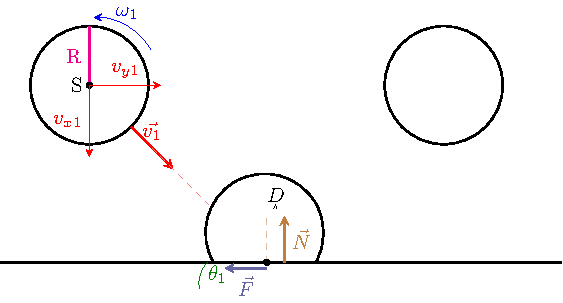
\includegraphics{diagram.pdf}\\
  \raggedright
  $\color{red}\vec{v_{1,2}}$ = rychlost před/po odrazu \\
  $\color{blue}\omega_{1,2}$ = spin před/po odrazu \\
  $\color[rgb]{0,0.5,0}\theta_{1,2}$ = úhel dopadu/odrazu \\
  
 \end{frame}

 \begin{frame}{Výzkumná otázka}
  \centering
  Jaký backspin je potřeba pro zpětný odraz míčku a jak ovlivňuje spin po
  odrazu? Pro všechny úhly odrazu
  ($\qty{0}{\degree}-\qty{90}{\degree}$) a vybrané
  rychlosti($\qty{1}{\meter\per\second} - \qty{10}{\meter\per\second}$).
 \end{frame}

 \section{Teorie} 

 \begin{frame}{Teorie}
  Triviální příklady:
  \begin{itemize}
   \item Když míček nepadá dolů nemá se od čeho odrazit 
   \item Bez úhlové rotace se úhel dopadu rovná úhlu odrazu
   \item Když míček letí rovnoběžně s povrchem nemůže se odrazit zpátky
   \item Když míček letí kolmo na povrch je velmi jednoduché aby se odrazil
    zpátky
  \end{itemize}
 \end{frame}

 \begin{frame}{Předpoklady}
 \begin{itemize}
  \item Deformuje se jen míček
  \item Popisujeme jen samotný odraz
  \item Normálová síla působí jen v jednom bodě
  \item Při odrazu dochází jen ke smýkání 
 \end{itemize}
\end{frame}

\section{Experimenty}

 \begin{frame}{Simulace}
 Pro materiálové konstanty relevantní pro golfový míček na žulovém povrchu:
 \[
  v_{x2} < 0 \Rightarrow \theta_1 > \qty{69}{\degree}
 \]
 Tedy směr odrazu není závislý ani na $v_{x1}$ ani na $\omega$.\\
 Dalším směrem mé práce je prozkoumat případy, kdy dochází i k rolování. Pro ty
 bude odpověď záležet i na jiných faktorech.
\end{frame}
\end{document}

